\documentclass{article}

\usepackage{amsfonts}
\usepackage{amsmath}
\usepackage{amssymb}
\usepackage{amsthm}
\usepackage{caption}
\usepackage{color}
\usepackage{enumerate}
\usepackage{fancyhdr}
\usepackage[margin=1in]{geometry}
\usepackage{hyperref}
\usepackage{graphicx}
\usepackage{latexsym}
\usepackage{listings}
\usepackage{mathrsfs}
\usepackage{natbib}
\usepackage[nottoc]{tocbibind}
\usepackage{setspace}
\usepackage{tikz}
\usepackage{tkz-graph}
\usepackage{url}

\providecommand{\all}{\ \forall \ }
\providecommand{\bs}{\backslash}
\providecommand{\e}{\varepsilon}
\providecommand{\E}{\ \exists \ }
\providecommand{\lm}[2]{\lim_{#1 \rightarrow #2}}
\providecommand{\m}[1]{\mathbb{#1}}
\providecommand{\mc}[1]{\mathcal{#1}}
\providecommand{\nv}{{}^{-1}}
\providecommand{\ov}[1]{\overline{#1}}
\providecommand{\p}{\newpage}
\providecommand{\q}{$\quad$ \newline}
\providecommand{\rt}{\rightarrow}
\providecommand{\Rt}{\Rightarrow}
\providecommand{\vc}[1]{\boldsymbol{#1}}
\providecommand{\wh}[1]{\widehat{#1}}

%\renewcommand\bibname{References}

\fancyhead{}
\fancyfoot{}
\fancyhead[R]{\thepage}
\fancyhead[C]{Landau}

\hypersetup{
    colorlinks,
    citecolor=black,
    filecolor=black,
    linkcolor=black,
    urlcolor=blue
}

\definecolor{dkgreen}{rgb}{0,0.6,0}
\definecolor{gray}{rgb}{0.5,0.5,0.5}
\definecolor{mauve}{rgb}{0.58,0,0.82}

\lstset{ 
 % basicstyle=\tiny,
  language=C,                % the language of the code
  numbers=none,
  numberfirstline=false,
  numbersep=5pt,                  % how far the line-numbers are from the code
  backgroundcolor=\color{white},      % choose the background color. You must add \usepackage{color}
  showspaces=false,               % show spaces adding particular underscores
  showstringspaces=false,         % underline spaces within strings
  showtabs=false,                 % show tabs within strings adding particular underscores
  frame=lrb,                   % adds a frame around the code
  rulecolor=\color{black},        % if not set, the frame-color may be changed on line-breaks within not-black text 
  tabsize=2,                      % sets default tabsize to 2 spaces
  captionpos=t,                   % sets the caption-position 
  breaklines=true,                % sets automatic line breaking
  breakatwhitespace=false,        % sets if automatic breaks should only happen at whitespace
  %title=\lstname,                   % show the filename of files included with \lstinputlisting;
  keywordstyle=\color{blue},          % keyword style
  commentstyle=\color{gray},       % comment style
  stringstyle=\color{dkgreen},         % string literal style
  escapeinside={\%*}{*)},            % if you want to add LaTeX within your code
  morekeywords={*, ...},               % if you want to add more keywords to the set
  xleftmargin=0.053in, % left horizontal offset of caption box
  xrightmargin=-.03in % right horizontal offset of caption box
}

\DeclareCaptionFont{white}{\color{white}}
\DeclareCaptionFormat{listing}{\parbox{\textwidth}{\colorbox{gray}{\parbox{\textwidth}{#1#2#3}}}}
\captionsetup[lstlisting]{format = listing, labelfont = white, textfont = white}
 %For caption-free listings, comment out the 3 lines above
 \lstset{frame = single}


%%% TITLE AND DATE

\title{\vspace{4cm} \hrule  \vspace{0.4cm} \huge
Dynamic Ledger: a tutorial
\vspace{0.4cm} \hrule}
\date{\today}


%%% DOCUMENT

\begin{document}
\begin{titlepage}

\maketitle

\begin{center}
\vspace{1cm}
\Large
\begin{center}
Will Landau \\ $\quad$ \\
Department of Statistics \\
Iowa State University \\ $\quad$ \\
\end{center}

\vfill
\large
Copyright \copyright ~Will Landau 2013. 
\end{center}
\end{titlepage}

\newpage 
\pagestyle{fancy}
\setcounter{page}{1}
\pagenumbering{roman}
\tableofcontents 

\newpage
\setcounter{page}{1}
\pagenumbering{arabic}
%\fancyhead[C]{\thesection}

\begin{flushleft}

\section{Introduction}

\paragraph{} Dynamic Ledger is a program for managing personal finances. Unlike most other accounting programs, it gives you control over your finances even when you have several delayed transactions. With it, you can be exactly as frugal as you need to be, and you can easily avoid spending more than you actually have. In addition, you can use the program to clean and condense your ledgers to save space.


\section{Installation}

\paragraph{} See {\tt INSTALL} for the standard installation instructions for any Linux/Unix package that uses GNU {\tt autotools}. Although standard, these instructions are cryptic and verbose, so I attempt to provide a simplified version below. 

\subsection{Requirements}
\begin{enumerate}
\item Make sure you have a C compiler on your system. Linux users can download and install gcc, the GNU Compiler Collection, at \url{http://gcc.gnu.org/}. Mac users can install gcc or clang through Xcode. Just open Xcode, go to Preferences $>$ Downloads, and look under the ``Compnents" tab. There you should be able to install the ``command line tools". Windows users should install Cygwin (cygwin.com) or MinGW (mingw.com) and get gcc during the installation.
\item Open a command line interface tool. Linux users should already be familiar with this Mac users should go open Applications $>$ Utilities $>$ Terminal. Windows users should open Cygwin (cygwin.com) or MinGW (mingw.com). You should have a basic familiarity with the Linux/Unix command line interface before you begin. If not, watch the tutorial at \url{http://www.youtube.com/watch?v=2FiQSLdnBqA} or any other linux command line tutorial and follow along with your own command line. At minimum, you should know the commands, {\tt cd}, {\tt ls}, and {\tt pwd}.
\end{enumerate}


\subsection{Installation}
\begin{enumerate}
\item Download and unzip the tarball, {\tt dl-0.0.tar.gz}, if you have not done so already. To unzip, ``cd" into the directory containing the tarball and enter into the command line,

\begin{lstlisting}
$ tar -zxvf dl-0.0.tar.gz
\end{lstlisting}

A directory called {\tt dl-0.0} should have been created.

\item ``cd" into {\tt dl-0.0} and enter the following into the command line.

\begin{lstlisting}
$ ./configure
$ make
$ sudo make install
\end{lstlisting}

You may have to type in your computer's password.
\end{enumerate}

\subsection{Check your installation}

At this point, your program should be ready to use. To test, type

\begin{lstlisting}
$ dl
\end{lstlisting}

{\tt dl} is the command you will type into the command line to use Dynamic Ledger. \q

For quick usage information, just type

\begin{lstlisting}
$ man dl
\end{lstlisting}

Use the up and down arrow keys to browse the documentation, and type ``q" to quit. 

\subsection{View source code documentation}

\paragraph{} Optionally, to view the documentation of the source code, use {\tt doxygen} (\url{http://www.stack.nl/~dimitri/doxygen/}). First, download and install {\tt doxygen}. Then open your command line interface program, ``cd" into the main directory of this package, and run

\begin{lstlisting}
$ doxygen Doxyfile
\end{lstlisting}

Standard {\tt doxygen} documentation is output to the {\tt html/}, {\tt latex/}, and {\tt rtf/} folders.


\section{Program usage}

\paragraph{} Let's use the ledger file, {\tt ledger.txt}, in the {\tt tutorial/} folder:

\begin{lstlisting}[title=ledger.txt]
amount    status  credit     bank        partition    description
-30.14    cp      card       checking    gas          gas
-15.36            card       checking    food         food
-5                card       checking                 paper
400                          checking
300                          checking    food
300                          checking    food
350                          checking    food
100                          checking    gas
800                          checking    gas
200                          checking    gas
400                          checking
440                          checking
\end{lstlisting} \q
 
You can type {\tt man dl} into the command line to learn what everything in this ledger file means, and you can read Section \ref{sec:file} to see an extended example. For now, let's just say that {\tt ledger.txt} is a tab-delimited spreadsheet where you record your financial transactions.

\subsection{Summarizing ledgers}

\paragraph{} To summarize {\tt ledger.txt}, open your command line interface program, ``cd" (change directories) into the directory containing {\tt ledger.txt}, and type

\begin{lstlisting}
$ dl ledger.txt
\end{lstlisting} 

\paragraph{} The following summary should print to your screen.

\begin{center}
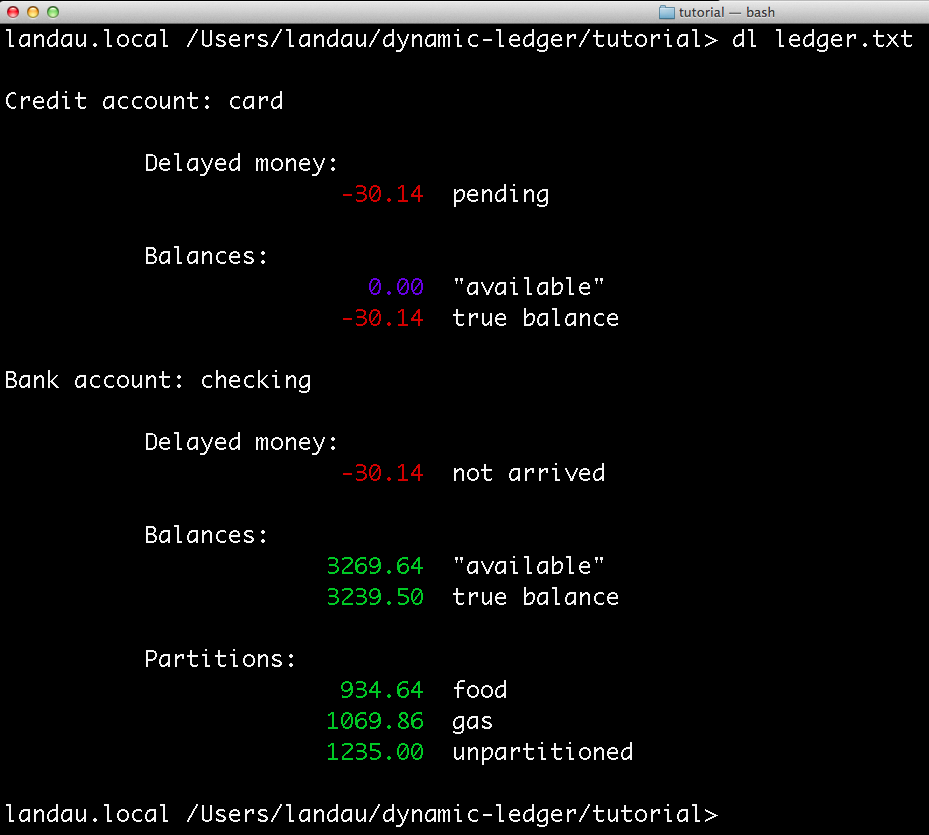
\includegraphics[scale=.45]{fig/usage0.png}
\end{center} 

\paragraph{} As Section \ref{sec:file} explains, this summary shows the balances of all the accounts in the ledger. Specifically, it predicts the balances that you should see when access your credit and bank accounts online (the ``available" balances), along with what your account balances \emph{will be} once all your delayed transactions have cleared (the true balances). 

\paragraph{} This feature is the real power of Dynamic Ledger. Just by looking at the summary, you can

\begin{enumerate}
\item Check that your ledger file is correct: i.e., verify that the ``available" and pending balances in the summary agree with the balances you see online.
\item Look at the true balances to see exactly how much \emph{real money} you have left to spend. That way, you can be sure to only spend money that you actually have.
\end{enumerate}

\clearpage

\subsection{Cleaning ledger files}

\paragraph{} Sometimes, ledger files get long and messy. With Dynamic Ledger, you can condense and clean them up. Let's say {\tt ledger.txt} looks like this: 

\begin{lstlisting}[title=ledger.txt]
amount    status  credit     bank        partition    description
-15.36    cp      card       checking    food         food

-5                card       checking                 paper
400                          checking
-30.14    cn      card       checking    gas          gas
300       l                  checking    food
300                          checking    food


350                          checking    food
100                          checking    gas
800                          checking    gas
200                          checking    gas
400                          checking

440                          checking
\end{lstlisting} \q

To output a condensed, clean version of this ledger to {\tt out.txt}, just type \q

\begin{lstlisting}
$ dl ledger.txt out.txt
\end{lstlisting} 

The condensed ledger looks like

\begin{lstlisting}[title=out.txt]
amount    status  credit     bank        partition    description
-30.14    cn      card       checking    gas          gas
-15.36    cp      card       checking    food         food
1235.00           card       checking                 condensed
300       l                  checking    food    
650.00                       checking    food         condensed
1100.00                      checking    gas          condensed
\end{lstlisting} 

\paragraph{} If you have read Section \ref{sec:file}, you will see that this operation summed up all the transaction amounts of the cleared transactions within each bank account partition and stored these sums as individual rows. The upshot is that you have a new, condensed ledger with your delayed and locked transactions still visible. You can verify that the summary of {\tt ledger.txt} is the same as the summary of {\tt out.txt} by typing \q

\begin{lstlisting}
$ dl ledger.txt
$ dl ledger.txt out.txt
$ dl out.txt
\end{lstlisting} 

\paragraph{} Type {\tt man dl} into the command line and read Section \ref{sec:file} to understand delayed transactions. You can specify the kind of delay of each transaction by entering ``cn", ``cp", ``c", ``p", or ``n" in the ``status" column of the ledger file. The condense/clean operation will leave these transactions alone. 

\paragraph{} In addition, you can lock any cleared transaction that you want preserved. Just enter ``l" into the status column. Then, the condense/clean operation will ignore it even though it is cleared.



\section{How to write and maintain a ledger file} \label{sec:file}

\paragraph{} Dynamic Ledger requires you to keep your ledger in a tab-delimited spreadsheet file. This section shows you how to keep track of your transactions in this ledger file when you're using the program to balance your checkbook.

\subsection{Managing delayed transactions over time}

\paragraph{} Suppose I have two bank accounts. I began with \$800 in my first bank account, and then I make a withdrawal of \$300. Suppose it's still too early for the \$300 withdrawal to show up on my bank account's website. In addition, I have a second bank account of \$1000. I make the following tab-delimited ledger file to record this information.

\paragraph{} Let's start with the following tab-delimited ledger file, {\tt ledger.txt}.

\begin{lstlisting}[title=ledger.txt]
amount    status	credit     bank        partition    description
-300      n                  bank1
800                          bank1
1000                         bank2
\end{lstlisting}

\paragraph{} The ``n" in the status column indicates that the \$300 charge has not arrived at bank1 yet. I can use Dynamic Ledger to compute the following summary of {\tt ledger.txt}.

\begin{center}
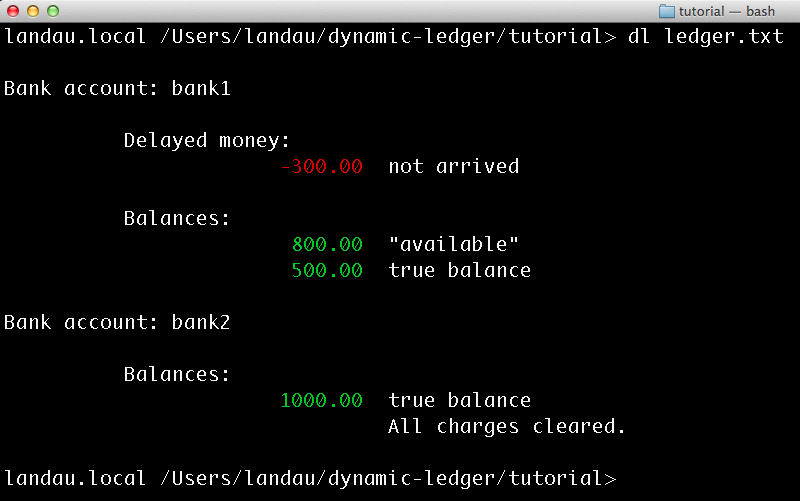
\includegraphics[scale=.45]{fig/sum0.png}
\end{center} 

\paragraph{} The program shows me an ``available" balance of \$800.00 because that is the balance I should see when I log on to my bank account's website to check. However, my true balance is \$500 because of the delayed \$300 withdrawal. 

\paragraph{} Suppose that next time I log on to my bank account's website, the \$300 withdrawal is shown as ``pending". To make {\tt ledger.txt} agree with what I see online, I change the ``n" status to ``p":

\begin{lstlisting}[title=ledger.txt]
amount    status	credit     bank        partition    description
-300      p                  bank1
800                          bank1
1000                         bank2
\end{lstlisting}

\paragraph{} The summary from Dynamic Ledger is now

\begin{center}
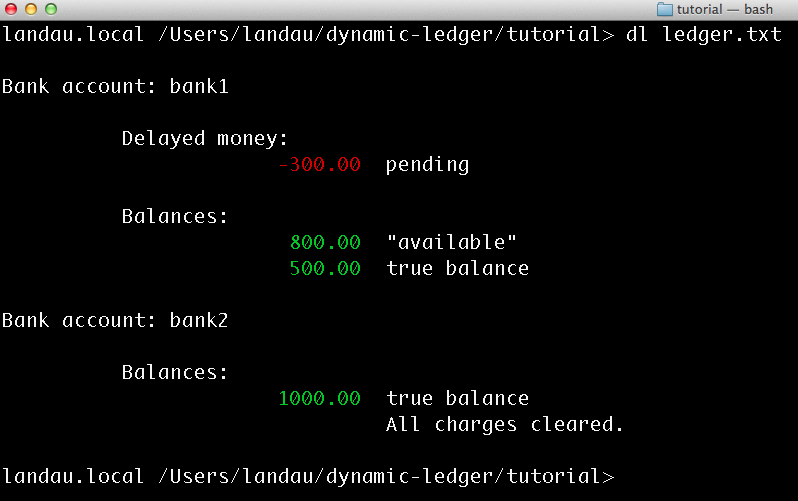
\includegraphics[scale=.45]{fig/sum1.png}
\end{center}  

\paragraph{} When the withdrawal finally clears online, I can delete the ``p":

\begin{lstlisting}[title=ledger.txt]
amount    status	credit     bank        partition    description
-300                         bank1
800                          bank1
1000                         bank2
\end{lstlisting}

\paragraph{} The summary from Dynamic Ledger is now

\begin{center}
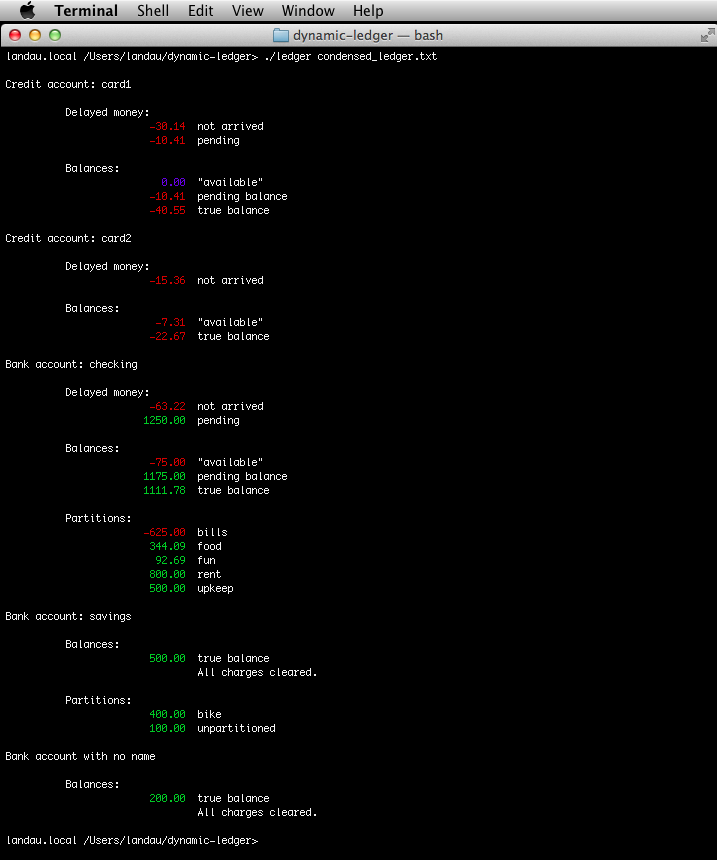
\includegraphics[scale=.45]{fig/sum2.png}
\end{center}  





\subsection{Managing credit accounts}

\paragraph{} Under the program's conceptual model, transactions flow through credit accounts into bank accounts. To see how this works, consider the following extended example. Suppose I start with a checking account with \$800. I spend \$5 on paper, then \$15.36 on food, and then \$30.14 on gas. I pay all those things with a credit card, but it's too early for any of those transactions to actually show up my credit card's website. I make the following tab-delimited ledger file.

\begin{lstlisting}[title=ledger.txt]
amount    status	credit     bank        partition    description
-30.14    cn      card       checking                 gas
-15.36    cn      card       checking                 food
-5        cn      card       checking                 paper
800                          checking
\end{lstlisting}

\paragraph{} Note the ``cn" transaction status code for all three charges. That means I made these transactions with a credit card, but it's too early for the charges to actually show up on the credit account's website. The summary of the ledger is \q

\begin{center}
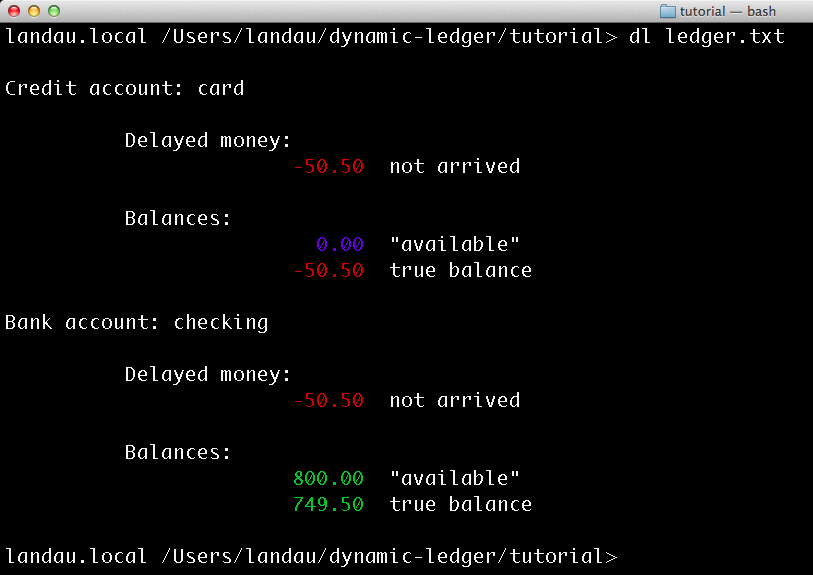
\includegraphics[scale=.45]{fig/sum3.png}
\end{center} 

\paragraph{} Notice that my credit card has an ``available" balance of \$0.00, but my true balance is -\$50.50. That means that when I go on online, I should see an account balance of  \$0.00 (if I recorded my transactions correctly). However, because I have delayed transactions, I owe the credit company \$50.50 in reality. Similarly, my bank account should show an ``available" balance of \$800.00 online, but in reality, I only have \$749.50 left to spend. 

\paragraph{} Over time, transactions will begin clear on the credit card company's website. Suppose that after a few days I see that the food and paper transactions have cleared, but the gas transaction is still ``pending". I change my transaction status codes to reflect the changes.

\begin{lstlisting}[title=ledger.txt]
amount    status	credit     bank        partition    description
-30.14    cp      card       checking                 gas
-15.36    c       card       checking                 food
-5        c       card       checking                 paper
800                          checking
\end{lstlisting}

\paragraph{} ``cp" means pending on the credit card, while ``c" means charged to the credit card but unpaid. The new summary from the program looks like \q

\begin{center}
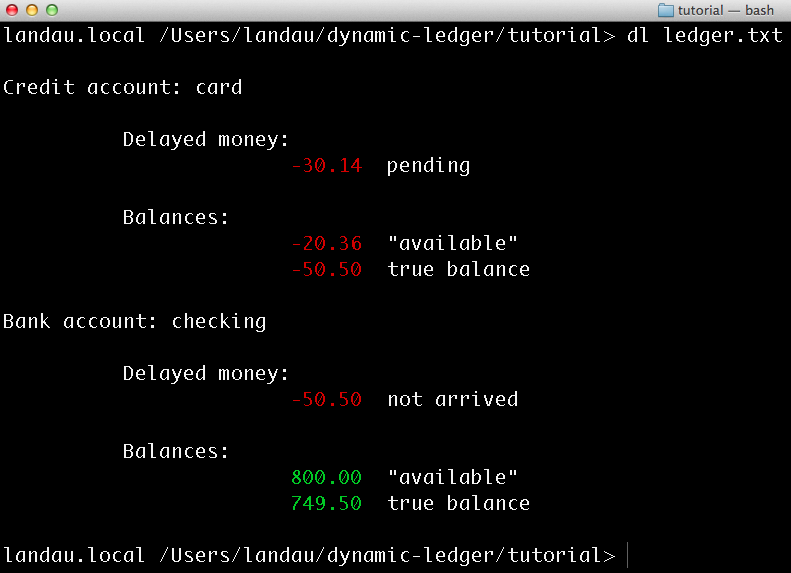
\includegraphics[scale=.45]{fig/sum4.png}
\end{center} 

\paragraph{} Since some charges have cleared, I can now make a credit card payment. I now pay my ``available" debt of \$20.36. (I cannot pay for pending charges). I now think of the food and paper transactions as a single charge of \$20.36 en route to my checking account. When I make the payment and it clears on the credit company's website, I update the ledger file.

\begin{lstlisting}[title=ledger.txt]
amount    status	credit     bank        partition    description
-30.14    cp      card       checking                 gas
-15.36    n       card       checking                 food (cred pmnt $20.36)
-5        n       card       checking                 paper (cred pmnt $20.36)
800                          checking
\end{lstlisting}

\paragraph{} The ``n" statuses means that the credit payment has not shown up on my bank account's website yet. The summary from the program is now \q

\begin{center}
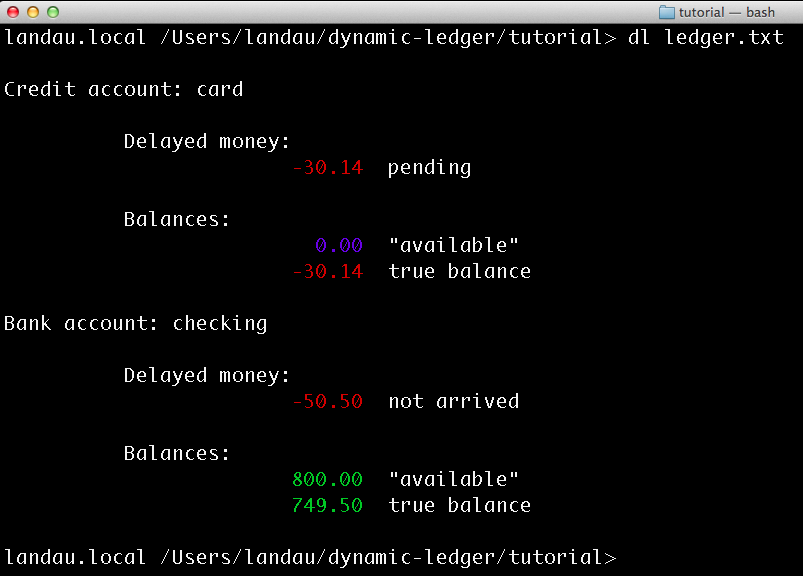
\includegraphics[scale=.45]{fig/sum5.png}
\end{center} \q

\paragraph{} I wait a day or two, and then I log on again and see that my credit card payment shows up as ``pending". Now, I change the n's to p's.

\begin{lstlisting}[title=ledger.txt]
amount    status	credit     bank        partition    description
-30.14    cp      card       checking                 gas
-15.36    p       card       checking                 food (cred pmnt $20.36)
-5        p       card       checking                 paper (cred pmnt $20.36)
800                          checking
\end{lstlisting}

\paragraph{} My summary shows

\begin{center}
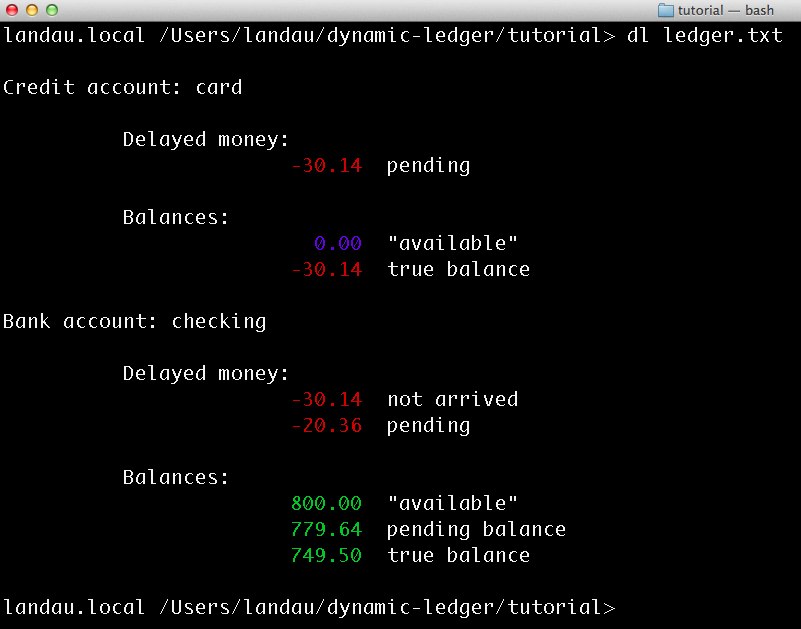
\includegraphics[scale=.45]{fig/sum6.png}
\end{center} \q

\paragraph{} Finally, when the credit card payment clears, I can delete the p's to show that the food and paper charges have completely cleared all my accounts.

\begin{lstlisting}[title=ledger.txt]
amount    status	credit     bank        partition    description
-30.14    cp      card       checking                 gas
-15.36            card       checking                 food (cred pmnt $20.36)
-5                card       checking                 paper (cred pmnt $20.36)
800                          checking
\end{lstlisting}

\paragraph{} My updated summary is now

\begin{center}
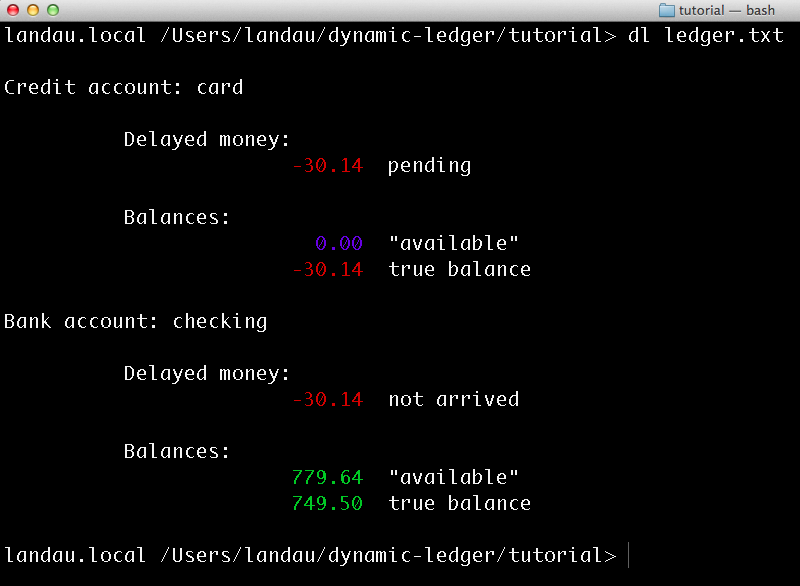
\includegraphics[scale=.45]{fig/sum7.png}
\end{center} \q



\subsection{Partitioning bank accounts}

\paragraph{} The program lets the user divide bank accounts into partitions. For example, if I make special partitions in my bank account for food and gas, I might write

\begin{lstlisting}[title=ledger.txt]
amount    status	credit     bank        partition    description
-30.14    cp      card       checking    gas          gas
-15.36            card       checking    food         food (cred pmnt $20.36)
-5                card       checking                 paper (cred pmnt $20.36)
400                          checking    
300                          checking    food
100                          checking    gas
\end{lstlisting}

\paragraph{} And my summary would look like 

\begin{center}
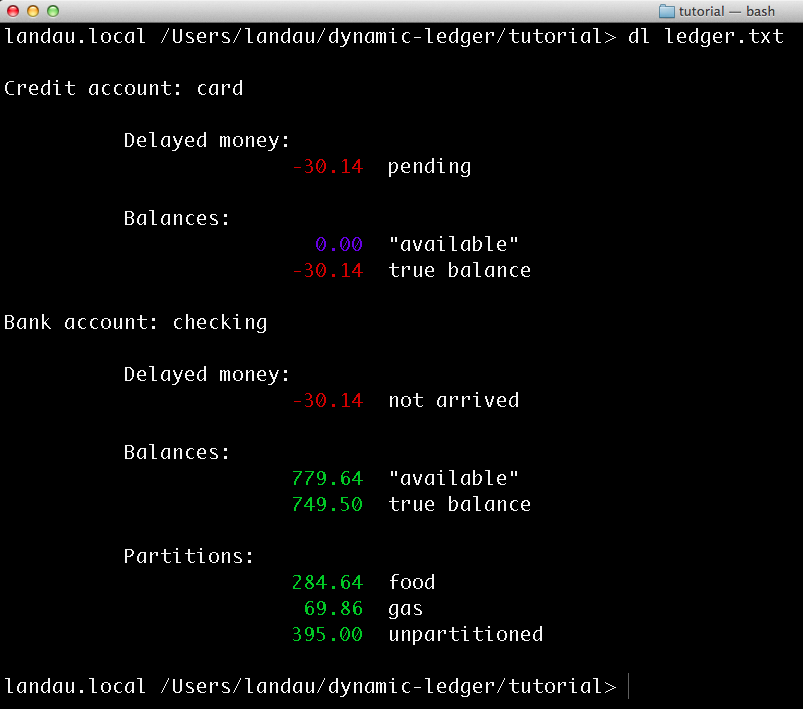
\includegraphics[scale=.45]{fig/sum8.png}
\end{center} \q

\paragraph{} Notice that only the true final balances for the partitions are shown. In other words, partition balances are calculated as if all transactions have completely cleared. This feature encourages you to avoid spending more money than you actually have.

\end{flushleft}
%\newpage 
%\bibliographystyle{plainnat} 
%\bibliography{}
\end{document}